\documentclass[12pt]{article}

\usepackage{ctex}

\usepackage{amsmath}    % 数学公式
\usepackage{siunitx}    % 物理量和单位

\usepackage{graphicx}
\graphicspath{{figures/}}   % 图片所在文件夹

% 去掉图/表编号与题注文字之间的冒号，改为两个空格
\usepackage{caption}
\DeclareCaptionLabelSeparator{twospace}{~~}
\captionsetup{labelsep=twospace}

\usepackage{geometry}   % 设置页边距
\geometry{a4paper, hmargin=2.54cm, vmargin=3.18cm}

\usepackage{setspace}   % 设置行距
\onehalfspacing         % 1.5 倍行距

\begin{document}
\section{行内公式与行间公式}
% 无序列表（itemize环境）示例
% 与之相对，enumerate 环境可产生有序列表
\begin{itemize}
    \item 行内公式：由一对 \verb|$| 包裹，或者 \verb|\(| 与 \verb|\)| 包裹。
    \item 行间公式：由一对 \verb|$$| 包裹，或者 \verb|\[| 与 \verb|\]| 包裹。
\end{itemize}

爱因斯坦质能方程是$E=mc^2$，也是
\[
    E=mc^2
\]

在 \LaTeX 中，用 \verb|^| 和 \verb|_| 标明上下标。

上下标的内容通常需用花括号（\verb|{ }|）包裹，否则只对后面的\textbf{一个符号}起作用。
\[
    e^x+y \neq e^{x+y}
\]

\section{数学模式的特点}

\subsection{公式内间距调整}

对于方程 $ax^2+bx+c=0$（$a \neq 0$），若$\Delta=b^2-4ac > 0$，则它的两个实数根为
\[
    x_1 = \frac{-b+\sqrt{\Delta}}{2a}, \quad x_2 = \frac{-b-\sqrt{\Delta}}{2a}
\]

\begin{itemize}
    \item 分式：\verb|\frac{分子}{分母}|。
    \item 根式：\verb|\sqrt[n]{f(x)}|。其中，可选参数$n$表示开$n$次方根。例如：\(\sqrt[3]{x}\)。
\end{itemize}

\subsection{正体、斜体、粗体和向量}
在量子力学中，微观粒子在势场 \(V(\mathbf{r})\) 中的运动可以描述为
\[
    \mathrm{i} \hbar \frac{\partial \Psi}{\partial t} = 
    - \frac{\hbar^2}{2m} \nabla^2 \Psi + V(\mathbf{r}) \Psi
\]
其中，\(\mathbf{r}\) 也可以写成 \(\vec{r}\)。

\section{物理量及其单位}

\subsection{手动调整}

单摆的运动周期为$T = 1.35 \;\mathrm{s}$.

小球转动惯量的理论值为
\[
J_{c,\text{理论}}=\frac{1}{10}mD^2
=3.32 \times 10^{-6} \; \mathrm{kg \cdot m^2}
\]

\subsection{使用siunitx宏包}

单摆的运动周期为$T = \SI{1.35}{s}$.

小球转动惯量的理论值为
\[
J_{c,\text{理论}}=\frac{1}{10}mD^2
=\SI{3.32e-6}{kg.m^2}
\]

我们也可以使用 \verb|\num{}| 命令将数字转化为科学技术法表示。例如，\verb|\num{3.32E-6}| 对应的输出为 \num{3.32E-6}。

\section{练习使用数学公式识别工具}

给出图~\ref{fig:math-formula-exercises} 所示的数学公式的\LaTeX{}代码。

\begin{figure}[htbp]
    \centering
    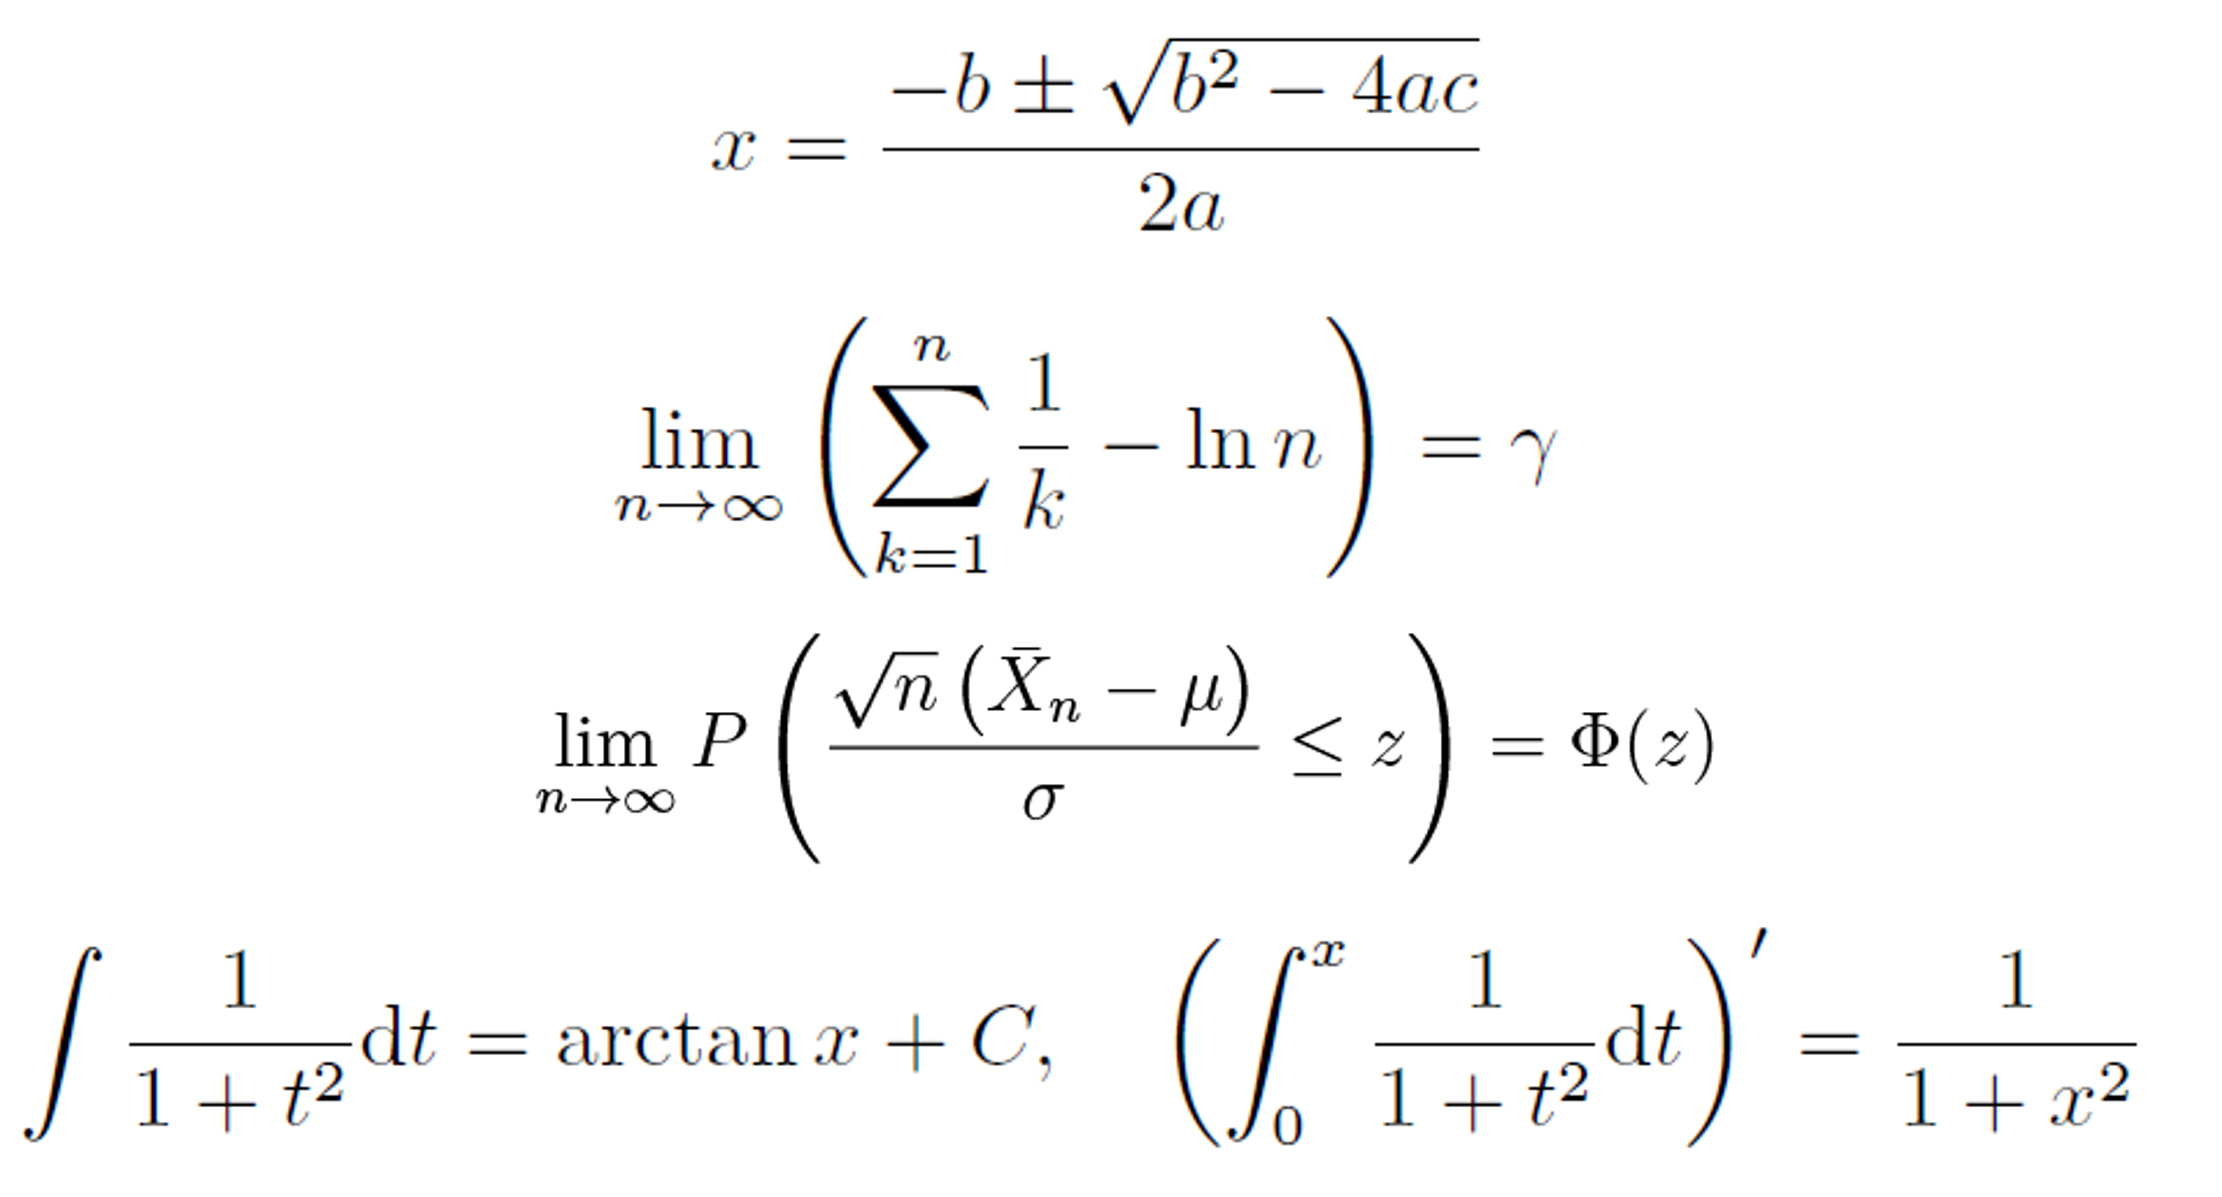
\includegraphics[width=0.8\linewidth]{math-formula-exercises.jpg}
    \caption{数学公式识别练习}
    \label{fig:math-formula-exercises}
\end{figure}

注意到括号高度与其中的内容适应，我们可以用一对 \verb|\left(| 与 \verb|\right)| 实现。

  
\end{document}
